\documentclass[aspectratio=169]{beamer}

% Advanced font selection for XeLaTeX and LuaLaTeX
\usepackage{fontspec}

% Add support for Romanian
\usepackage{polyglossia}
\setdefaultlanguage{romanian}

% Support for interactive hyperlinks
\usepackage{hyperref}
\hypersetup{
  colorlinks,
  linkcolor=,
  citecolor=blue,
  urlcolor=blue
}

% Bibliography management support
\usepackage[doi=false,isbn=false,url=false,maxbibnames=3]{biblatex}
\renewcommand*{\bibfont}{\scriptsize}

\addbibresource{references.bib}

% Support for inserting images
\usepackage{graphicx}

\graphicspath{{./figures/}}

% Unified shell escape interface
\usepackage{shellesc}

% Support for drawing beautiful figures
\usepackage{tikz}

% Support for externalizing TikZ figures (for caching)
\usetikzlibrary{external}
\tikzexternalize[prefix=cache/]

% Ensure cache directories exist and forward -output-directory to child lualatex runs
\newcommand{\tikzexternaloutdirflag}{}

% tex-fmt: off
\directlua{
  local outdir = status.output_directory
  local function ensure_dir(path)
    local acc = path:sub(1, 1) == "/" and "/" or ""
    for part in path:gmatch("[^/]+") do
        acc = (acc == "" or acc == "/") and (acc .. part) or (acc .. "/" .. part)
        lfs.mkdir(acc)
    end
  end
  function _G.ensure_tikz_cache_dir(filename)
    local base = (outdir and outdir ~= "") and (outdir:gsub("/+$", "") .. "/cache/") or "cache/"
    local dir = filename:match("^(.*)/[^/]+$")
    ensure_dir(dir and (base .. dir) or base)
  end
  ensure_tikz_cache_dir("")
  if outdir and outdir ~= "" then
    token.set_macro("tikzexternaloutdirflag", '-output-directory="' .. outdir .. '" ')
  end
}
% tex-fmt: on

\tikzset{
  external/system call={%
    lualatex \tikzexternalcheckshellescape -halt-on-error -interaction=batchmode \tikzexternaloutdirflag -jobname "\image" "\texsource"%
  }
}


% Basic math commands
\usepackage{amsmath}
% Common mathematical symbols
\usepackage{amssymb}

% Advanced mathematical commands
\usepackage{mathtools}

% Encode mathematical symbols using Unicode characters
\usepackage[warnings-off={mathtools-colon,mathtools-overbracket}]{unicode-math}

% Based on https://tex.stackexchange.com/a/482560/263993
\newcommand{\inputtikz}[1]{%
  \directlua{ensure_tikz_cache_dir("\luaescapestring{#1}")}%
  \tikzsetnextfilename{#1}%
  \input{#1}%
}

% Change the default Beamer theme
\usetheme{Warsaw}

% Disable the rendering of navigation symbols in the bottom-right
\setbeamertemplate{navigation symbols}{}

% Disable list of sections in the header
\setbeamertemplate{headline}{}

% Add slide number to Warsaw's split footline
\setbeamertemplate{footline}{%
  \leavevmode%
  \hbox{%
    \begin{beamercolorbox}[wd=.5\paperwidth,ht=2.5ex,dp=1.125ex,leftskip=.3cm,rightskip=.3cm]{author in head/foot}%
      \usebeamerfont{author in head/foot}\hfill\insertshortauthor
    \end{beamercolorbox}%
    \begin{beamercolorbox}[wd=.5\paperwidth,ht=2.5ex,dp=1.125ex,leftskip=.3cm,rightskip=.3cm]{title in head/foot}%
      \usebeamerfont{title in head/foot}\insertshorttitle\hfill\insertframenumber
    \end{beamercolorbox}%
  }%
  \vskip0pt%
}

% Insert a title slide at the beginning of each new section
\AtBeginSection[]{
  \begin{frame}
    \vfill
    \centering
    \begin{beamercolorbox}[sep=8pt,center,shadow=true,rounded=true]{title}
      \usebeamerfont{title}\insertsectionhead\par%
    \end{beamercolorbox}
  \end{frame}
}

% Definitions of custom commands
% Differential symbol for integral
\newcommand*{\diff}{\symrm{d}}

% Absolute value and norm symbols.
% Code taken from https://tex.stackexchange.com/questions/43008/absolute-value-symbols
\DeclarePairedDelimiter\abs{\lvert}{\rvert}%
\DeclarePairedDelimiter\norm{\lVert}{\rVert}%

% Swap the definition of \abs* and \norm*, so that \abs
% and \norm resizes the size of the brackets, and the
% starred version does not.
\makeatletter
\let\oldabs\abs
\def\abs{\@ifstar{\oldabs}{\oldabs*}}
%
\let\oldnorm\norm
\def\norm{\@ifstar{\oldnorm}{\oldnorm*}}
\makeatother


% Presentation metadata
\title{Emisie superradiantă de lumină cu moment cinetic orbital}
\subtitle{prin împrăștierea Thomson inversă a unui fascicul laser Laguerre-Gauss de un mănunchi de electroni relativiști}
\author{Gabriel Majeri \and Mădălina Boca \and Virgil Băran}
\institute{
  Facultatea de Fizică \\
  Universitatea din București
}
\date{26 noiembrie 2026}

\begin{document}

\begin{frame}
  \titlepage

  \vskip-0.5cm

  \centering
  \small{
    Conferința Anuală de Comunicare a Rezultatelor Cercetării la UB
  }

  \vskip0.1cm
\end{frame}

\section{Introducere}

\begin{frame}
  \frametitle{Motivație}

  \begin{itemize}
    \item Lumina este o \textbf{oscilație transversă} a câmpului electromagnetic.
    \item La fel ca orice undă transversă, poate avea \textbf{moment cinetic} (\textit{angular momentum}), pe care îl descompunem într-o componentă datorată polarizării (\textbf{moment cinetic de spin}) și una datorată formei frontului de undă (\textbf{moment cinetic orbital}).
  \end{itemize}
\end{frame}

\begin{frame}
  \frametitle{Momentul cinetic al luminii}

  \begin{figure}
    \centering
    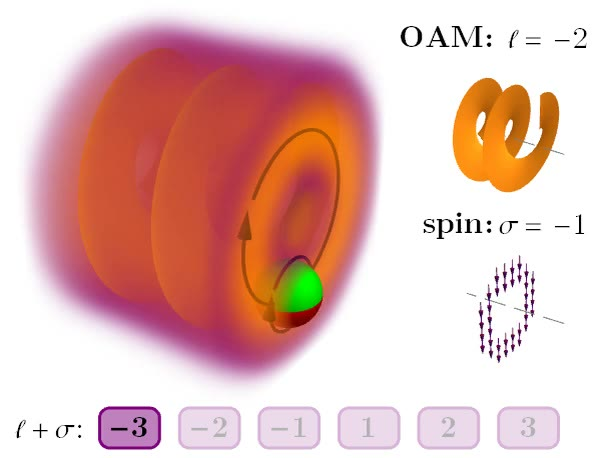
\includegraphics[width=0.75\textwidth]{figures/oam_vs_spin.jpg}
    \caption{Cadru dintr-un video de pe \href{https://en.wikipedia.org/wiki/File:OAM_vs_spin_video.ogg}{Wikipedia}, creat de Jozum Bjada}
  \end{figure}
\end{frame}

\begin{frame}
  \frametitle{Schema experimentală}

  \begin{figure}
    \centering
    \resizebox{\columnwidth}{!}{\inputtikz{figures/experiment_geometry.tex}}
    \caption{Reprezentare vizuală a metodei propuse. Un fascicul laser LG care se propagă în direcția \(-z\) lovește un mănunchi de electroni relativiști care se mișcă în direcția \(+z\). Radiația emisă este măsurată pe un detector aflat la o distanță \(Z\).}
  \end{figure}
\end{frame}

\begin{frame}
  \centering{
    \huge{Mulțumesc pentru atenție!}
  }
\end{frame}

\begin{frame}[allowframebreaks]
  \frametitle{Referințe}

  \printbibliography
\end{frame}

\section{Backup slides}

\begin{frame}
  \frametitle{Ecuațiile lui Maxwell}

  Undele pe care le studiem sunt soluții ale \textbf{ecuațiilor lui Maxwell} \cite{Maxwell1865,Jackson1999,Griffiths2023}:

  \begin{align*}
    &\symbf{\nabla} \cdot \symbf{E} = \frac{\rho}{\epsilon_0} \tag{Legea lui Gauss} \\[0.2em]
    &\symbf{\nabla} \times \symbf{E} = - \frac{\partial \symbf{B}}{\partial t} \tag{Legea lui Faraday} \\[0.2em]
    &\symbf{\nabla} \cdot \symbf{B} = 0 \\[0.2em]
    &\symbf{\nabla} \times \symbf{B} = \mu_0 \symbf{J} + \mu_0 \epsilon_0 \frac{\partial \symbf{E}}{\partial t} \tag{Ampère-Maxwell} \\[0.2em]
    &\symbf{F} = q \left(\symbf{E} + \symbf{v} \times \symbf{B}\right) \tag{Forța Lorentz}
  \end{align*}
\end{frame}


\end{document}
